\section{Jump Points}
In the previous section we developed simple rules for pruning neighbours during 
individual node expansions. We now extend this idea in order to define a 
macro-step operator which speeds up optimal search by selectively expanding
only certain nodes on a grid map. We term these nodes \emph{jump points}.
\par
The basic idea is straightforward: we give a simple example in Figure 
\ref{fig:jumppoints}(a).
Here we observe that when moving straight there are many cases where
the expanded node has only a single successor.
Since this successor cannot create or improve any nodes on the open list we 
propose to evaluate it immediately, thereby avoiding an unnecessary list
maintenance operation. 
If we keep moving in the same direction we can continue this process until we 
either reach a node with more than one successor (a jump point), which we add to the open list instead of the nodes whose evaluation we expedited, or we find an 
obstacle which indicates that further search in this direction is fruitless.
\par
In the remainder of this section we will develop a macro-step operator which 
speeds up node expansion by identifying jump point successors in the case of
both straight and diagonal moves. We begin by making precise the concept of a
jump point:

\begin{definition}
\label{def:jump}
A node $x$ is designated a jump point if it satisfies at least one of the following
conditions:
\begin{enumerate}
\item{$x$ is a node which, after pruning, is adjacent to at least one neighbour
whose evaluation is forced according to the rules in Section
\ref{sec:prunestraight} and Section \ref{sec:prunediagonal}.}
\item{$x$ is located on the same row or column of the grid as the goal.}
\item{$x$ has one or more successors which are themselves jump points.}
\end{enumerate}
\end{definition}

Note that we distinguish between a neighbour, which is immediately adjacent to
$x$ on the grid, and a successor which may not be. 
This is a fine but important distinction as in our work a neighbour can be a 
successor but the converse is not necessarily true.
Thus, when expand $x$, we will only consider its successors.


\subsection{Generating Successors}
The process by which we generate the set of successors necessary to expand a
node $x$ is given in Algorithm \ref{alg:successors}.
We start with the pruned set of neighbours immediately adjacent to $x$ (line 2).
Any neighbouring node $n$ whose inclusion into this set is forced, according the 
rules outlined in Section \ref{sec:prunestraight} and Section 
\ref{sec:prunediagonal}, is immediately generated as a successor for $x$ 
(lines 3:4).
We then attempt to defer the generation of each remaining neighbour by seeing if 
we can ``jump'' to another node further away from $x$ but lying in the same 
relative direction to $x$ as $n$ (lines 5:7). For example, if the edge $(x, n)$ constitutes a
straight move travelling \emph{right} from $x$, we look for a jump point among
the nodes immediately to the right of $x$.
If we find such a node, we add it to the set of successors instead of $n$.
In the case where we fail to find a jump point, we add nothing.
The process continues until the set of neighbours for $x$ is exhausted.

\input alg_jumpexpansion

\subsection{Jumping}
The process by which we identfy jump points is given in Algorithm
\ref{alg:jump}; it requires an initial node $x$, a direction of travel $dir$
(e.g. up, down, left right, etc) and the goal node $g$.
In rough overview, the algorithm attempts to establish whether $x$ has any 
jump point successors by iteratively stepping in a direction $dir$ and testing
if the node $n$ at that location satisfies the constraints outlined in 
Definition \ref{def:jump}.
When this is the case, $n$ is designated a jump point and returned (lines 5, 7
and 13).
When $n$ is not a jump node the algorithm recurses and steps again in direction
$dir$ but this time $n$ is the new initial node (lines 9, 12 and 14).
The recursion terminates when an obstacle is encountered and no further
steps can be taken (lines 1:3).
Note that before recursing diagonally the algorithm must first 
fail to detect any straight jump points (lines 10:13).
\par
%Consider Figure \ref{fig:jumppoints} where we illustrate this process by
%example.
%In the case of Figure \ref{fig:jumppoints}(a) $x$ is the initial node and the
%direction of travel is \emph{right}. The algorithm steps four times (recursing
%at line 9 each time) before
%encountering a successor $y$ which has a forced neighbour $z$; thus satisfying
%the first constraint of Definition \ref{def:jump}. $y$ is returned and becomes
%a successor of $x$.
%In the case of Figure \ref{fig:jumppoints}(b) the direction of travel is
%\emph{up-and-right}.
%Here the algorithm steps 3 times before encountering a node $y$ which is
%located on the same row as the goal node $g$; thus satisfying constraint 2 of
%Definition \ref{def:jump}.
%Notice however that before stepping diagonally (line 14) the algorithm 
%looks for jump points by stepping in the straight directions \emph{right} and
%\emph{up} (lines 11:13).
%This allows us to prove that no potential successors were missed and is
%criticial to retain optimality.

%\noindent
%Figure \ref{fig:pruningrules}(b) shows an example of jump point which satisfies the
%first condition of Defintion \ref{def:jump}: here we cannot apply Straight Pruning
%Rule 4 as the evaluation of neighbour 3 is forced.
%The same is true of the example in Figure \ref{fig:pruningrules}(d): we cannot
%apply Diagonal Pruning Rule 3 as the evaluation of neighbour 1 is forced.


\begin{figure}[tb]
       \begin{center}
		   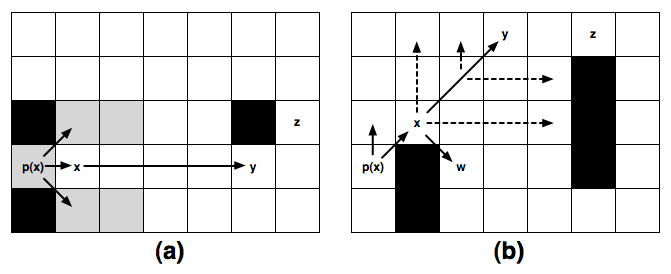
\includegraphics[scale=0.35, trim = 10mm 10mm 10mm 0mm]
			{diagrams/jumppoints.png}
       \end{center}
	\vspace{-3pt}
       \caption{Examples of straight (a) and diagonal (b) jump points.
Dashed lines indicate a sequence of interim node evaluations that reached
a dead end. Strong lines indicate eventual successor nodes.}
       \label{fig:jumppoints}
\end{figure}

\subsection{Optimality}

Sketch: show that each pruning rule discards only neighbours
which cannot belong to the optimal path for the problem at hand.
Then, by induction, demonstrate that jump points have the same 
property. 

Complications:
 - jump points when passing the row or column associated with the goal
 - no jump points at the top of a row/column ending in an obstacle.

